\resizebox{0.5\textwidth}{!}{%
	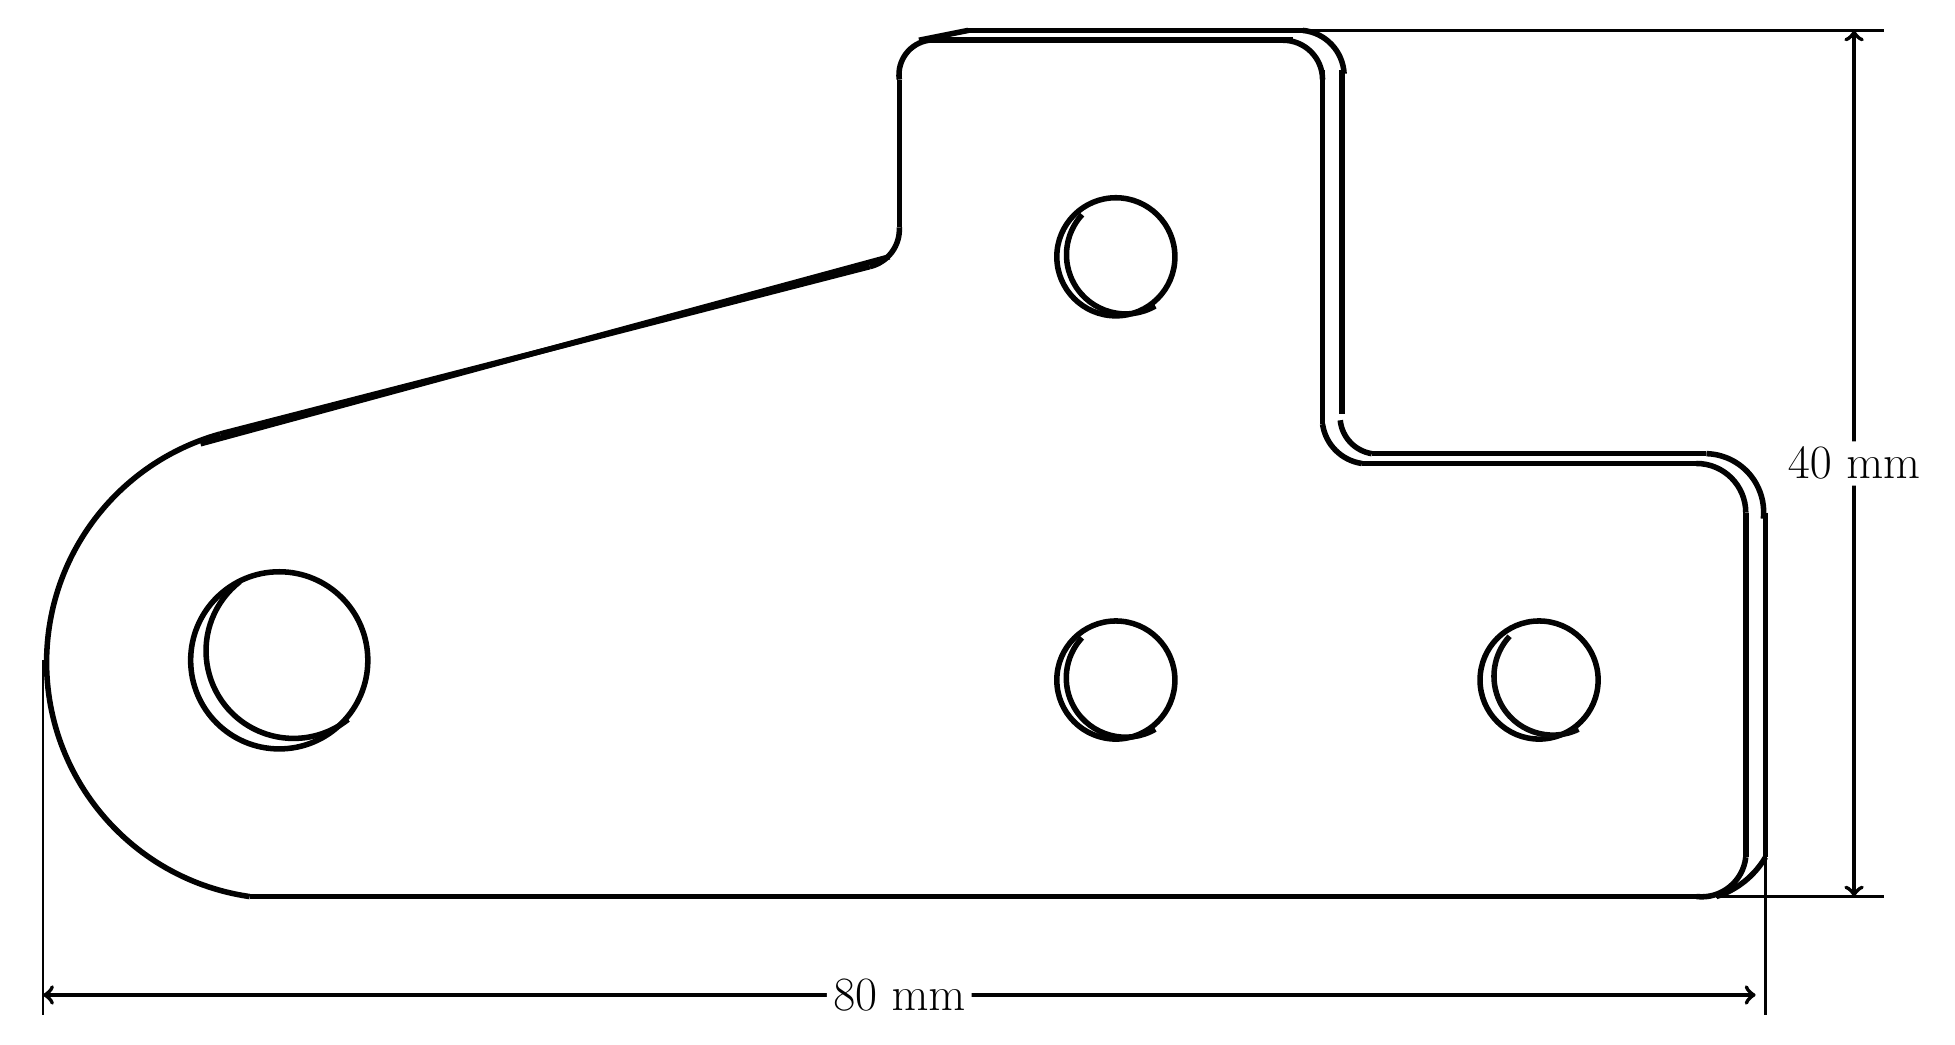
\begin{tikzpicture}
		\tikzstyle{every node}=[font=\fontsize{18.2pt}{23.7pt}\selectfont]
		
		\draw[color={rgb,255:red,2; green,2; blue,2}, draw opacity=1, line width=2pt] (-12.375,23.625) -- (-4.125,25.75);
		\draw[color={rgb,255:red,2; green,2; blue,2}, draw opacity=1, line width=2pt] (-3.75,28.125) -- (-3.75,26.25);
		\draw[color={rgb,255:red,2; green,2; blue,2}, draw opacity=1, line width=2pt] (-3.375,28.625) -- (1.25,28.625);
		\draw[color={rgb,255:red,2; green,2; blue,2}, draw opacity=1, line width=2pt] (1.625,28.25) -- (1.625,23.75);
		\draw[color={rgb,255:red,2; green,2; blue,2}, draw opacity=1, line width=2pt] (2.125,23.25) -- (6.375,23.25);
		\draw[color={rgb,255:red,2; green,2; blue,2}, draw opacity=1, line width=2pt] (7,22.625) -- (7,18.25);
		\draw[color={rgb,255:red,2; green,2; blue,2}, draw opacity=1, line width=2pt] (6.375,17.75) -- (-12,17.75);
		\draw[color={rgb,255:red,2; green,2; blue,2}, draw opacity=1, line width=2pt] (-12,17.75) arc[start angle=-98.18, end angle=-254.52, radius=3.0073];
		\draw[color={rgb,255:red,2; green,2; blue,2}, draw opacity=1, line width=2pt] (-3.75,26.25) arc[start angle=3.10, end angle=-76.84, radius=0.4865];
		\draw[color={rgb,255:red,2; green,2; blue,2}, draw opacity=1, line width=2pt] (-3.75,28.125) arc[start angle=-171.87, end angle=-261.87, radius=0.4419];
		\draw[color={rgb,255:red,2; green,2; blue,2}, draw opacity=1, line width=2pt] (1.125,28.625) arc[start angle=90.00, end angle=0.00, radius=0.5000];
		\draw[color={rgb,255:red,2; green,2; blue,2}, draw opacity=1, line width=2pt] (2.125,23.25) arc[start angle=-98.08, end angle=-171.92, radius=0.5886];
		\draw[color={rgb,255:red,2; green,2; blue,2}, draw opacity=1, line width=2pt] (6.375,23.25) arc[start angle=90.00, end angle=0.00, radius=0.6250];
		\draw[color={rgb,255:red,2; green,2; blue,2}, draw opacity=1, line width=2pt] (7,18.25) arc[start angle=-6.34, end angle=-96.34, radius=0.5660];
		
		\draw[color={rgb,255:red,2; green,2; blue,2}, draw opacity=1, line width=2pt] (-11.625,20.75) circle (1.125cm);
		\draw[color={rgb,255:red,2; green,2; blue,2}, draw opacity=1, line width=2pt] (-1,20.5) circle (0.75cm);
		\draw[color={rgb,255:red,2; green,2; blue,2}, draw opacity=1, line width=2pt] (-1,25.875) circle (0.75cm);
		\draw[color={rgb,255:red,2; green,2; blue,2}, draw opacity=1, line width=2pt] (4.375,20.5) circle (0.75cm);
		
		\draw[color={rgb,255:red,2; green,2; blue,2}, draw opacity=1, line width=2pt] (1.375,28.75) arc[start angle=84.39, end angle=2.75, radius=0.5812];
		\draw[color={rgb,255:red,2; green,2; blue,2}, draw opacity=1, line width=2pt] (1.375,28.75) -- (-2.875,28.75);
		\draw[color={rgb,255:red,2; green,2; blue,2}, draw opacity=1, line width=2pt] (-3.5,28.625) -- (-2.875,28.75);
		\draw[color={rgb,255:red,2; green,2; blue,2}, draw opacity=1, line width=2pt] (1.875,28.25) -- (1.875,23.875);
		\draw[color={rgb,255:red,2; green,2; blue,2}, draw opacity=1, line width=2pt] (2.25,23.375) -- (6.5,23.375);
		\draw[color={rgb,255:red,2; green,2; blue,2}, draw opacity=1, line width=2pt] (2.25,23.375) arc[start angle=-99.00, end angle=-174.30, radius=0.4774];
		\draw[color={rgb,255:red,2; green,2; blue,2}, draw opacity=1, line width=2pt] (7.25,22.625) -- (7.25,18.25);
		\draw[color={rgb,255:red,2; green,2; blue,2}, draw opacity=1, line width=2pt] (6.5,23.375) arc[start angle=88.54, end angle=-6.13, radius=0.7464];
		\draw[color={rgb,255:red,2; green,2; blue,2}, draw opacity=1, line width=2pt] (7.25,18.25) arc[start angle=-30.44, end angle=-72.24, radius=1.1220];
		\draw[color={rgb,255:red,2; green,2; blue,2}, draw opacity=1, line width=2pt] (-12.625,23.5) -- (-3.875,25.875);
		\draw[color={rgb,255:red,2; green,2; blue,2}, draw opacity=1, line width=2pt] (-10.75,20) arc[start angle=-51.53, end angle=-232.16, radius=1.1128];
		\draw[color={rgb,255:red,2; green,2; blue,2}, draw opacity=1, line width=2pt] (-0.5,25.25) arc[start angle=-60.03, end angle=-222.66, radius=0.7517];
		\draw[color={rgb,255:red,2; green,2; blue,2}, draw opacity=1, line width=2pt] (-0.5,19.875) arc[start angle=-59.95, end angle=-222.67, radius=0.7529];
		\draw[color={rgb,255:red,8; green,8; blue,8}, draw opacity=1, line width=2pt] (4.875,19.875) arc[start angle=-64.22, end angle=-222.69, radius=0.7479];
		
		\draw[color={rgb,255:red,2; green,2; blue,2}, draw opacity=1, line width=1pt] (-14.625,20.75) -- (-14.625,16.25);
		\draw[color={rgb,255:red,2; green,2; blue,2}, draw opacity=1, line width=1pt] (7.25,21) -- (7.25,16.25);
		\draw[color={rgb,255:red,2; green,2; blue,2}, draw opacity=1, line width=1pt] (1.375,28.75) -- (8.75,28.75);
		\draw[color={rgb,255:red,2; green,2; blue,2}, draw opacity=1, line width=1pt] (6.625,17.75) -- (8.75,17.75);
		
		\draw[color={rgb,255:red,2; green,2; blue,2}, draw opacity=1, line width=1.5pt, <->] 
		(8.375,28.75) -- (8.375,17.75)
		node[pos=0.5, fill={rgb,255:red,255; green,255; blue,255}, fill opacity=1, text opacity=1, inner xsep=0.080cm, inner ysep=0.085cm, rounded corners=0.020cm]{40 mm};
		
		\draw[color={rgb,255:red,2; green,2; blue,2}, draw opacity=1, line width=1.5pt, <->] 
		(-14.625,16.5) -- (7.125,16.5)
		node[pos=0.5, fill={rgb,255:red,255; green,255; blue,255}, fill opacity=1, text opacity=1, inner xsep=0.080cm, inner ysep=0.085cm, rounded corners=0.020cm]{80 mm};
		
	\end{tikzpicture}
}%